\chapter{Data visualization}
\label{cap:studio_data_viz}
\intro{In questo capitolo verrà presentata una panoramica della data visualization, spiegandone caratteristiche, usi e principi.
Viene inoltre proposto un metodo di classificazione dei grafici per ottimizzare le visualizzazioni.}\\

\section{Definizione e applicazioni}
\subsection{La necessità di rappresentare i dati}
%INTRO + CAP 1: “Design della mente – infografica e data viz” di Paolo Bottazini, Michele Gotuzzo
La visualizzazione dei dati ha una tradizione millenaria. Sin dagli albori della civiltà umana, 
le persone hanno sviluppato metodi per rappresentare visivamente i dati al fine di renderli più facili da comprendere, 
memorizzare e trasmettere.
Negli ultimi decenni, tuttavia, questa esigenza ha conosciuto un incremento senza precedenti.

Viviamo infatti nell'epoca dell'\emph{information overload} e dei \emph{big data}, dove le informazioni
arrivano con una velocità, un volume e una varietà così travolgenti che non siamo in grado di comprenderli se non attraverso
un ulteriore strato di astrazione.
Tale rivoluzione si deve soprattutto allo sviluppo delle tecnologie digitali, grazie alle quali siamo arrivati a disporre di una quantità 
apparentemente infinita di informazioni, tra sapere sociale, motori di ricerca e volontà delle persone di esprimersi.

In questo contesto, la \emph{data visualization} è diventata fondamentale per interpretare e trarre intelligenza da questa grande mole di dati.
Nello specifico, essa consente di fissare l'attenzione in segni maneggevoli - le rappresentazioni grafiche - che consentono una lettura dell'informazione
semplice e intuitiva. Tramite tali segni, è possibile cogliere funzioni strutturali e relazioni impreviste tra fenomeni, oltre che scoprire regolarità che 
altrimenti sarebbero rimaste nascoste, facilitando eventuali risoluzioni e valutazioni.

\bigskip
\noindent Possiamo dunque definire la \emph{data visualization} come l'insieme dei meccanismi di traduzione dei dati in rappresentazioni grafiche
mediante i quali l'informazione viene resa più chiara ed efficace. Più specificamente, 
potremmo dire che è un processo di traslazione dei dati all'interno di un contesto visivo atto ad amplificarne la cognizione.


\subsection{Obiettivi della data visualization}
%cap 6: https://onlinelibrary.wiley.com/doi/book/10.1002/9781119209560
Gli obiettivi alla base della \emph{data visualization} sono:
\begin{itemize}
    \item \textbf{Identificare}, ovvero trovare un dataset significativo, né troppo banale né troppo complesso, da cui sia possibile
    ricavarne delle informazioni utili;
    \item \textbf{Manipolare}, ossia analizzare e combinare i dati in modo da chiarirne il significato;
    \item \textbf{Formattare}, ovvero standardizzare il modo con cui si accede ai dati per una consumazione più efficiente;
    \item \textbf{Presentare}, ossia rappresentare i dati formattati in modo da esprimerne il significato nascosto.
\end{itemize}
\noindent Si desidera dunque massimizzare l'efficacia ed efficienza della visualizzazione dell'informazione. Ciò comporta:
\begin{itemize}
    \item Per quanto riguarda l'efficienza: ridurre la complessità e il rumore e nella visualizzazione che sono non necessari e potrebbero
    portare addirittura a correlazioni incorrette.
    \item Per quanto riguarda l'efficacia: fornire informazioni comprensibili e utili in modo che sia possibile prendere decisioni informate in base a esse.
\end{itemize}

\bigskip
%https://infogram.com/blog/what-is-data-visualization/?_gl=1*1rypyyw*_up*MQ..*_ga*MTg5MzY2NzU2MS4xNzE5MzMxMTgw*_ga_LD50PRQER7*MTcxOTMzMTE3OS4xLjAuMTcxOTMzMTE3OS4wLjAuMA..
\noindent Il fine ultimo di questi obiettivi è quello di:
\begin{itemize}
    \item Rendere i dati comprensibili e memorabili,
    \item Facilitare nuove scoperte e individuare trend e valori anonimi,
    \item Visualizzare velocemente relazioni e regolarità nei dati,
    \item Rendere migliore e più consapevole la presa di decisioni e stimolare la formulazione di ulteriori domande più specifiche.
\end{itemize} 


\subsection{Applicazioni}
Nell'età contemporanea, il processo di visualizzazione dei dati è ormai diventato essenziale per la gestione quotidiana di qualsiasi 
impresa, governo e organo informativo.

Imprese e pubbliche amministrazioni sfruttano la \emph{data visualization} per comprendere meglio la propria organizzazione e 
prendere decisioni più informate basate sui dati, ad esempio per quanto riguarda la gestione delle risorse e lo sviluppo di strategie future. 
Questo approccio, inoltre, è cruciale anche per la percezione esterna dell'organizzazione e dunque per contraddistinguersi da enti a lei analoghi.

Alla stessa maniera, anche per gli organi informativi (e.g. i giornali) la \emph{data visualization} è diventata indispensabile. 
Infatti, solo grazie a essa è possibile ricavare delle intuizioni altrimenti impossibili e rendere fruibili 
tali risultati in maniera chiara e intuitiva. Ciò risulta particolarmente importante per tali organi in quanto la loro mission è proprio diffondere 
e comunicare informazioni.



\section{Principi e linee guida}
\subsection{Creare visualizzazioni efficaci}
%https://infogram.com/blog/what-is-data-visualization/?_gl=1*1rypyyw*_up*MQ..*_ga*MTg5MzY2NzU2MS4xNzE5MzMxMTgw*_ga_LD50PRQER7*MTcxOTMzMTE3OS4xLjAuMTcxOTMzMTE3OS4wLjAuMA..
Una buona visualizzazione nasce dall'incontro di comunicazione, data science e design.
% immagine da https://venngage.com/templates/diagrams/data-viz-edf4207a-7fb4-47ce-ae1e-df730cc93d78 ma rifatta
\begin{figure}[!h] 
    \centering 
    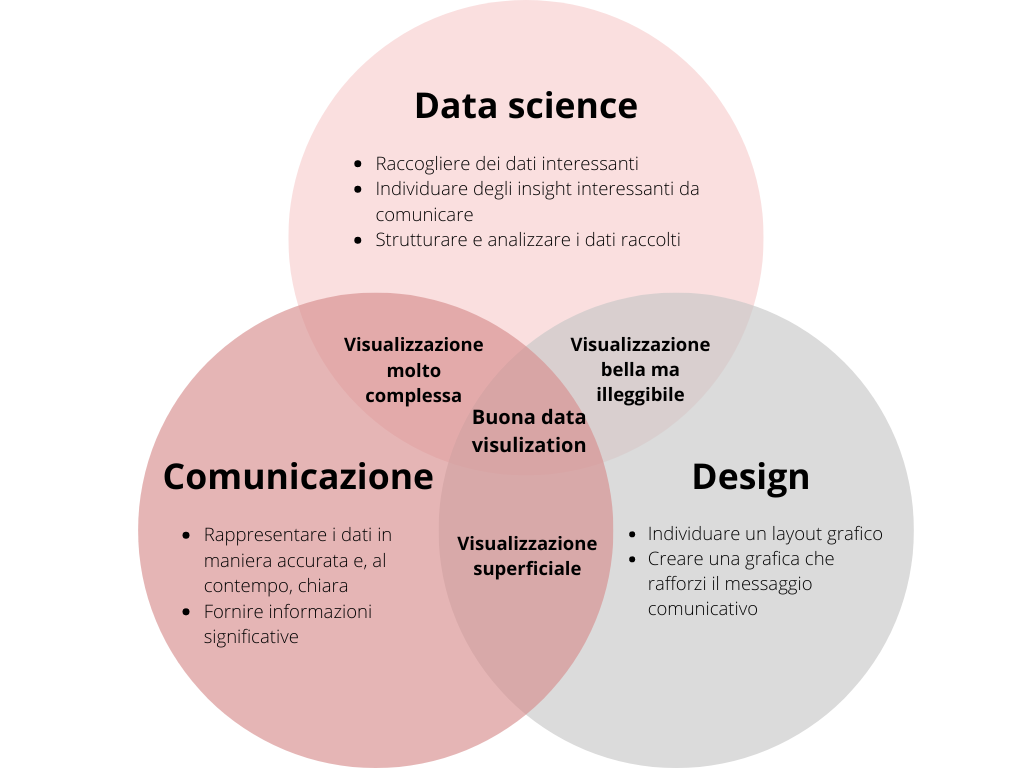
\includegraphics[width=0.8\columnwidth]{data-viz/venn_good_dataviz} 
    \caption{Diagramma di Venn: intersezione tra data science, comunicazione e design nella visualizzazione dei dati}
    \label{fig:venn_good_dataviz}
\end{figure}

\noindent Se realizzata correttamente, infatti, essa è capace di ricavare da dataset complessi delle informazioni significative e trasmetterle in maniera intuitiva.
Usando le parole di Edward Tufte, statistico e luminare nel campo della \emph{data visualization}, una visualizzazione dei dati eccellente consiste in
``idee complesse comunicate con chiarezza, precisione ed efficienza''.
% TODO: aggiungere citazione come footnote (%“The visual Display of Quantitative Information” di Edward R. Tufte, CAP 1: Graphical excellence)

%cap1: “L'arte funzionale – Infografica e visualizzazione delle informazioni” di Alberto Cairo
Da ciò ne consegue che l'obiettivo della \emph{data visualization} e ruolo di un architetto dell'informazione è quello di rendere il più efficiente possibile il processo che il cervello
umano compie nell'acquisire conoscenza e saggezza a partire dall'osservazione di fenomeni.
Tale processo può essere descritto, in maniera semplificata, attraverso la cosiddetta gerarchia DIKV (\emph{Data-Information-Knowledge-Wisdom}) di seguito riportata.
\begin{figure}[!h] 
    \centering 
    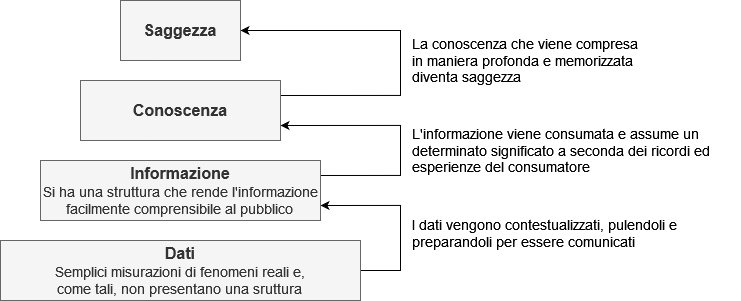
\includegraphics[width=\columnwidth]{data-viz/DIKV} 
    \caption{Gerarchia DIKV}
    \label{fig:DIKV}
\end{figure}

Come si nota subito dall'immagine \ref{fig:DIKV}, è essenziale ottenere dati puliti, completi e rappresentativi (responsabilità della data science). Solo successivamente sarà possibile rappresentare tali dati e 
ottenere una conoscenza valida (responsabilità di comunicazione e design).

\bigskip
%“L'arte funzionale – Infografica e visualizzazione delle informazioni” di Alberto Cairo
% cap 2
\noindent Nella visualizzazione dei dati in sé, bisogna tener conto innanzitutto che la forma grafica delle informazioni non è di per sé un'applicazione artistica; infatti, 
essa deve anche coadiuvare il fruitore in attività intellettive. Pertanto, la forma deve aspirare a oggettività, precisione e, soprattutto, funzionalità.
Per descrivere tale principio, possiamo dunque prendere in prestito le parole di Louis Sullivan sull'architettura modernista del XX secolo: ``La forma segue la funzione''. 
Tale massima può infatti essere applicata anche all'architettura dell'informazione nel contesto della \emph{data visualization}, giacché
un complesso di dati può assumere più forme, ma non tutte le forme sono sempre adatte e usabili. Infatti, la loro scelta deve dipendere dal
tipo di dati e obiettivo della rappresentazione. Ne consegue che più preciso è lo scopo, più limitata sarà la gamma di forme tra cui scegliere.

Il processo di decisione della rappresentazione grafica viene meglio approfondito nella sezione \ref{sec:classificare_grafici}.

\bigskip
\noindent Una volta decisa la forma migliore, bisogna comunque adattarla alla visualizzazione del caso specifico attraverso delle scelte di design.
In tal senso, si può adottare un approccio più minimalistico, promosso dal sopracitato Edward Tufte, o un approccio più ``artistico'', 
sostenuto da Nigel Holmes, famoso grafico specializzato nel design delle informazioni.

%“The visual Display of Quantitative Information” di Edward R. Tufte
%CAP 1: Graphical excellence
Per Tufte è essenziale combinare una semplicità di design a complessità dei dati. Per lui, il fruitore della visualizzazione deve poter ricavare il maggior numero di idee e informazioni dal minor uso possibile di spazio e inchiostro.
A tal proposito, egli sviluppa le seguenti formula: 
\begin{center}
    $\text{Rapporto dati-inchiostro} = \frac{\text{inchiostro usato per la codifica dei dati}}{\text{inchiostro totale usato per la stampa del grafico}}$
\end{center}
\begin{center}
    $\text{Densità dei dati} = \frac{\text{numero di voci in una matrice di dati}}{\text{area occupata dal grafico}}$            %CAP 8: Data density and small multiples
\end{center}
% TODO: aggiungere footnote che questa parte si intende solo quella dei datiDensità = number entries in una matrice di dati / area del grafico.
%Meglio se è più alta (mappe è altissima), risulta anche essere più affidabile. Bisogna comunque evitare di sovrappopolare lo spazio, in quel caso conviene utilizzare tecniche di data-reduction (averaging, clustering, smoothing).
%Attenzione! Stiamo parlando della parte di dati, per quanto riguarda la parte non strettamente riguardante questi (chartjunk) meglio meno.
evidenziando che più il rapporto è alto, migliore è la rappresentazione. Ciò implica che sia necessario evitare di utilizzare tutti gli elementi decorativi o, più in generale, tutte le parti che possono essere omesse 
senza perdere dati, ovvero tutto ciò che Tufte chiama ``chartjunk'' (e.g. la maggior parte delle griglie e sfondi posti sotto i grafici).

%“L'arte funzionale – Infografica e visualizzazione delle informazioni” di Alberto Cairo
%cap 3
D'altra parte, Holmes sostiene che ci si può divertire con la forma, purché la funzione principale rimanga comunicare i dati. Infatti, ciò che Tufte potrebbe considerare ``chartjunk'', e dunque superfluo,
potrebbe invece rivelarsi utile a facilitare la memoria e dunque portare alla saggezza. Holmes segue dunque la linea di pensiero del filosofo austriaco Otto Neurath, padre dell'\emph{Isotype}, il quale sostiene che 
``il soggetto della mostra deve essere serio ma va combinato con un fascino e un richiamo diretto per tutti''.
% TODO: citazione footnote? “From Hyeroglyphics to Isotype”

%“L'arte funzionale – Infografica e visualizzazione delle informazioni” di Alberto Cairo
%Cap 4
Qualsiasi approccio si decida di intraprendere, rimane comunque essenziale sfruttare lo spazio a disposizione per ricercare la profondità, seppur rimanendo nei limiti dettati dal tipo di fruitori.
Tale profondità si concretizza quasi sempre tramite la rappresentazione di dati multivariati, che consentono l'analisi di un fenomeno in maniera più accurata. %multivariato da %“The visual Display of Quantitative Information” di Edward R. Tufte, CAP 1: Graphical excellence
Le informazioni non devono infatti essere semplificate o snellite dalla visualizzazione, bensì devono essere solamente chiarite. La rappresentazione dovrebbe permettere dunque di suscitare riflessioni non superficiali ed evidenziare tendenze, pattern 
o realtà altrimenti invisibili. 
Solo in un secondo momento ci si può dedicare all'estetica della presentazione, utilizzando gli spazi rimanenti. Tale precauzione è da prendere affinché i dati ricevano subito tutto lo spazio necessario ed eventuali
effetti speciali o decorazioni siano inseriti solo se ne presenta l'opportunità.


\subsection{Linee guida}
%“The visual Display of Quantitative Information” di Edward R. Tufte
%CAP 1: Graphical Integrity
Nel visualizzare dati è necessario garantire che le informazioni siano rappresentate accuratamente e senza distorsioni.
A tal scopo, è dunque necessario perseguire un'integrità grafica. Ciò implica l'uso di:
\begin{itemize}
    \item proporzioni corrette tra la rappresentazione dei numeri sul grafico e le quantità numeriche fornite, come pure tra il 
    numero di dimensioni rappresentate graficamente e il numero delle variabili nei dati;
    \item scale appropriate che mostrino la vera variazione dei dati (e.g. scale con intervalli regolari);
    \item etichette dettagliate e chiare che non forviino l'utente;
    \item elementi che contestualizzino il grafico.
\end{itemize}

%“The visual Display of Quantitative Information” di Edward R. Tufte
%CAP 9: AESTHETICS AND TECHNIQUE IN DATA GRAPHICAL DESIGN
\noindent Come accennato precedentemente, altrettanto importante è la scelta del design. Ciò include:
\begin{itemize}
    \item La scelta di un formato e layout appropriato, scegliendo la combinazione di frasi, tabelle
    e grafici che meglio mostri la riflessione che si vuole comunicare (e.g. per più di due numeri, conviene usare una tabella piuttosto che una frase). Ciò comporta:
    \begin{itemize}
        \item per l'occidente, un orientamento (specie per quanto riguarda il testo) che va dall'alto a sinistra verso il basso a destra;
        \item l'uso di grafici corredati da piccoli messaggi di chiarimento, piuttosto che spiegazioni sparse.
    \end{itemize}
    \item L'uso simbiotico, coerente e diretto di parole, numeri e figure.
    \item Visualizzare i dati in maniera accessibile, anche e soprattutto per quanto riguarda dettagli di dati complessi. Ciò comporta:
    \begin{itemize}
        \item l'uso di codifiche non troppo elaborate, che non necessitino il continuo controllo della legenda;
        \item nel caso di grafico con colori, la scelta di quest'ultimi compiuta in modo tale da tenere in considerazione anche le persone daltoniche e color-deficient;
        \item l'uso di caratteri leggibili.
    \end{itemize}
\end{itemize}



\section{Classificare i grafici}\label{sec:classificare_grafici}
Lo sviluppo e disponibilità al pubblico di nuovi strumenti avanzati ha consentito anche ad utenti non esperti di visualizzare dati ed estrarne informazioni dettagliate, 
permettendo loro di creare grafici e diagrammi.
Tuttavia, persiste ancora un ampio divario di conoscenza tra questi utenti e i modelli visivi esistenti.
Ne consegue che spesso le forme visive scelte per la rappresentazione non sono le più efficaci essendo limitate da un ristretto numero di opzioni conosciute.
In alcuni casi, addirittura, il formato visivo scelto risulta essere anche poco comprensibile o fuorviante per il caso d'uso specifico.

Senza una classificazione chiara, diventa dunque difficile per questo tipo di utenti selezionare la tecnica di visualizzazione più adeguata.
Nelle seguenti sezioni, si esaminano dunque dei criteri di classificazione identificati, assieme a uno strumento prototipale che mira ad 
automatizzare questo processo di classificazione.

\subsection{Metodo di classificazione}
I criteri principali da tenere in considerazione nella scelta del grafico sono:
\begin{itemize}
    \item l'obiettivo della visualizzazione,
    \item i tipi di dati disponibili.
\end{itemize}

\subsubsection{Obiettivi della visualizzazione}
Quando parliamo di ``obiettivo della visualizzazione'' intendiamo il tipo di relazione tra i dati che vogliamo mettere in evidenza attraverso
la rappresentazione grafica. I principali obiettivi individuati sono:
\begin{itemize}
    \item \textbf{Divergenza}, quando si vuole mettere in luce le differenze di valori a partire da un punto fisso (solitamente lo 0, ma può essere
    ad esempio anche una media).
    \begin{itemize}
        \item Esempio: confrontare la produttività del turno di mattina con quello del turno di sera.
    \end{itemize}
    \item \textbf{Correlazione}, quando si vuole enfatizzare la relazione tra due o più variabili. In questi casi, il fruitore della visualizzazione assumerà che le 
    variabili coinvolte siano in relazione causale, pertanto se così non fosse è necessario specificarlo.
    \begin{itemize}
        \item Esempio: esplorare come la qualità del sonno influenzi le prestazioni accademiche.
    \end{itemize}
    \item \textbf{Ranking}, quando si vuole mostrare la posizione degli elementi rispetto agli altri e il loro valore effettivo passa in secondo piano.
    \begin{itemize}
        \item Esempio: mostrare i dieci paesi con il tasso di inquinamento più alto.
    \end{itemize}
    \item \textbf{Distribuzione}, quando si vogliono mostrare eventuali pattern nei dati, evidenziando valori ed eventi di un dataset e quando si verificano. 
    \begin{itemize}
        \item Esempio: mostrare la frequenza di incidenti stradali per tipo di veicolo.
    \end{itemize}
    \item \textbf{Cambiamento nel tempo}, quando si vogliono enfatizzare dei trend che variano nel tempo.
    \begin{itemize}
        \item Esempio: analizzare come l'uso dei social media è cambiato negli ultimi cinque anni.
    \end{itemize}
    \item \textbf{Composizione}, quando si vuole mostrare come una singola entità viene suddivisa nelle sue componenti.
    \begin{itemize}
        \item Esempio: mostrare la composizione delle emissioni di gas serra per settore industriale.
    \end{itemize}
    \item \textbf{Grandezze}, quando si vogliono comparare grandezze, che siano esse assolute (per un maggior livello di dettaglio) o relative. 
    \begin{itemize}
        \item Esempio: mostrare la dimensione del mercato degli smartphone in termini di volumi di vendita.
    \end{itemize}
    \item \textbf{Spazi}, quando si vogliono mostrare pattern geografici o posizioni precise.
    \begin{itemize}
        \item Esempio: mostrare i paesi con la maggiore concentrazione di risorse naturali.
    \end{itemize}
    \item \textbf{Flussi}, quando si vogliono mostrare volumi o intensità con cui si passa tra due o più stati o condizioni.
    \begin{itemize}
        \item Esempio: esplorare la rete di interconnessioni finanziarie tra le banche globali.
    \end{itemize}
\end{itemize}

\subsubsection{Tipi di dati}
Una prima distinzione nel tipo di dati riguarda:
\begin{itemize}
    \item \textbf{dati numerici},
    \item \textbf{dati categorici}.
\end{itemize}
Il dataset fornito per la visualizzazione potrà dunque essere composto da dati tutti numerici, tutti categorici oppure da un mix dei due.

\bigskip
\noindent Un'altra distinzione si ha tra:
\begin{itemize}
    \item \textbf{dati univariati}, quando ho un dataset molto piccolo composto da una sola variabile;
    \item \textbf{dati multivariati}, quando ho un dataset composto da più variabili.
\end{itemize}

\bigskip
\noindent In base alle suddette classificazioni, si può specificare ulteriormente il tipo di dato:
\begin{itemize}
    \item In caso di dataset con multiple variabili numeriche:
    \begin{itemize}
        \item \textbf{dati ordinati}, dove è presenta almeno una variabile numerica che è ordinata;
        \item \textbf{dati non ordinati}, dove l'ordine non è presente.
    \end{itemize}
    \item In caso di dataset con multiple variabili categoriche:
    \item \begin{itemize}
        \item \textbf{dati ordinati},
        \item \textbf{dati ordinati},
        \item \textbf{dati non ordinati}.
    \end{itemize}
    \item In caso di almeno 
\end{itemize}


% TODO: dire che non per tutti gli obiettivi, ci possono essere tutti tipi di dato e aggiungere 
% sviluppata questa classificazione e riportare grafici (?)


\subsection{Chart-chooser}
%file criteri_scelta_grafico_v0.1.0 + codice + prompt LLM
%fonte: https://www.data-to-viz.com/ e https://ft-interactive.github.io/visual-vocabulary/
\subsubsection{Analisi dei dati}
\subsubsection{Individuazione dell'obiettivo}
\subsubsection{Proposta di grafici}






